\chapter{Einleitung}\label{ch:einleitung}
Vor mehr als fünfzig Jahren wurde der erste IBM Großrechner, das sog. System/360, vorgestellt.
Seit dieser Zeit setzen sich die monolitisch aufgebauten Systeme in Bezug auf Leistungsfähigkeit und Zuverlässigkeit gegenüber
anderen Systemen ab.(Kommentar: tun sie das? Vorschlag: seit dieser Zeit stehen diese Systeme (auch "Mainframes" genannt) für hohe
Leistungsfähgikeit und Zuverlässigkeit und hosten bis heute weltweit geschäftskritischen Worlkoad bei Banken, Versicherungen, 
Behörden usw.). 
(Kommentar: erwähnen z/OS und die Middlewareprodukte CICS, DB2 MQ), Hardware z15
Neben der kontinuierlichen Weiterentwicklung der Hardware und Prozessortechnologie änderte sich auch die Art und  Weise, wie Software für Großrechnersysteme entwickelt wurde über die Jahre drastisch.
Zu Beginn wurden Programme auf Lochkarten (ABBILDUNG !!) gestanzt und umständlich über ein Lesegerät eingelesen.
(Hinweis auf verwendete Programmiersprachen, COBOL ASM)
Heute stehen dem Entwickler moderne IDE´s (Kommentar: Erklärung? Link? Glossar?) zur Verfügung, um mit neuen Sprachen (Java) Anwendungen
für z/OS zu entwickeln.
Trotz dieser Veränderungen verlor der Mainframe im Zug der Dezentralisierung der IT hinzu Client-Server-Umgebungen in den 1990-er Jahren an Bedeutung. 
(Kommentar: Seit den 90ern verliert er in der IT Lehre (?)  an Bedeutung, oder "geht der Trend weg von..."... , im EInsatz hat er ja nach wie vor eine hohe Bedeutung...) 
Dieser Prozess führte soweit, dass in den frühen 1990-er Jahren bereits Vorhersagen über die Abschaltung des letzten Mainframes getroffen wurden.\footnote{\cite{Alsop.1993}}
\cite{Ceruzzi.2003}
(Kommentar: Heutzutage muss sich der Mainframe in die Cloud-Welt integrieren, tut das insb. durch zLinux.

Trotz dieser Vorhersagen (Kommentar: wird doppelt verwendet... vielleicht Nichtdestotrotz) verarbeiten heutzutage z/OS basierte Großrechnersysteme weltweit circa 1,2 Millionen CICS\footnote{Begrifferklärung zu CICS in \ref{cics}} Transaktionen pro Sekunde.\footnote{\cite{IBM.2019}} (Kommentar:  z.B. als Backend von Geldautomaten.
Im Vergleich hierzu werden 63.000 Google Suchanfragen pro Sekunde abgesetzt. \footnote{\cite{Sullivan.2016}}

Wie hat es diese schon seit den frühen 1990-er Jahren totgesagte Technologie geschafft auch heute noch diese Relevanz zu haben?
Hier kommen die klar definierten Vorteile und Use-Cases des Mainframes zum Tragen.
(Kommentar: das folgende geht hier für eine Einleitung meiner Meinung nach zu tief... vlt. reicht es hier eine Erwühnung von Stabilität, Verfügbarkeit, Security. 
Zunächst ist `RAS`\footnote{reliability, availability and serviceability} zu nennen.
Dies beschreibt grundsätzlich, die Stabilität eines Hard- und Softwaresystems.
Hierzu zählt vor allem das Verhalten bei einem Hardware-/Softwaredefekt und möglichst automatische Erkennung und möglichst effektive Behebung von diesen.
Zusätzlich sollte dies keinen oder nur selten einen kompletten Systemausfall zur Folge haben.
\begin{figure}[h]
	\centering
	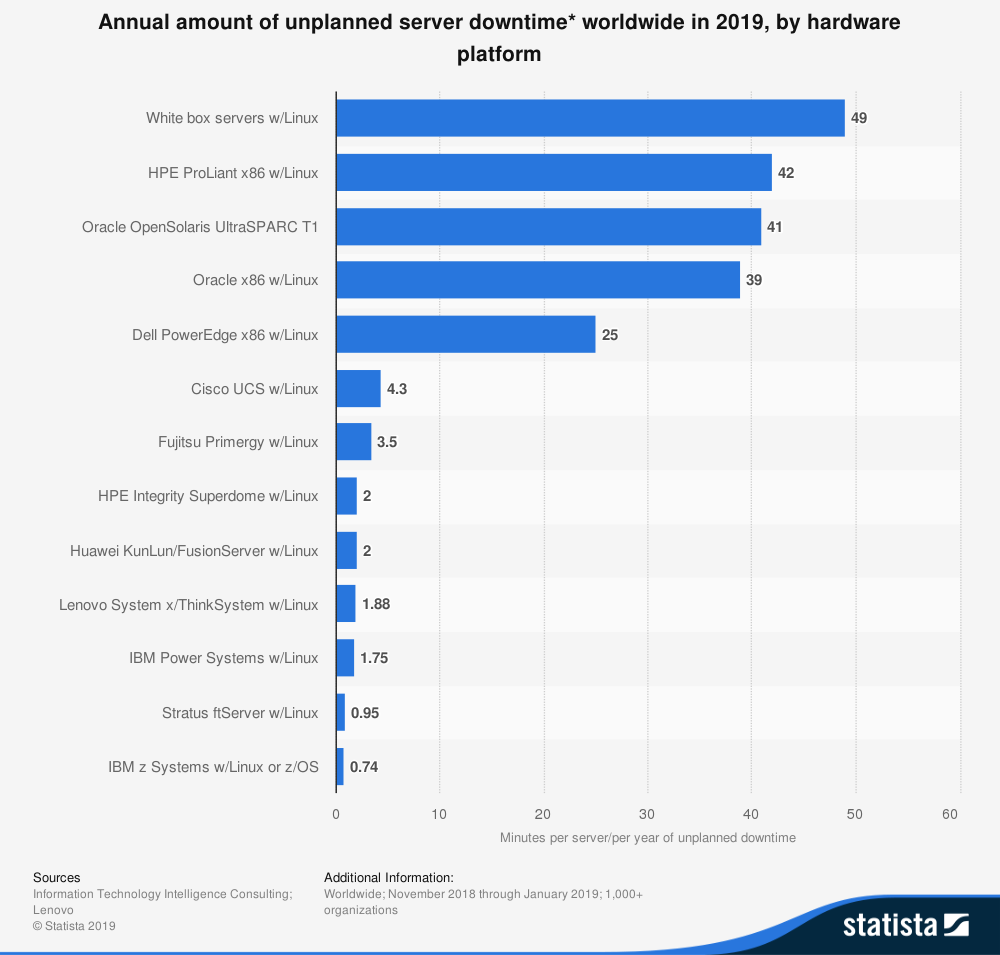
\includegraphics[width=\textwidth]{figures/statistic_id515285_unplanned-server-downtime-globally-2019-by-hardware-platform.png}
	\caption{Annual amount of unplanned server downtime worldwide in 2019, by hardeware platform}
	\label{fig:serverdowntime}
\end{figure}
Abbildung \ref{fig:serverdowntime} zeigt die ungeplante Server Ausfallzeit in Minuten pro Server im Jahr 2019.
Wie zu sehen ist, schneidet der IBM z Systems w/Linux oder z/OS, das Mainframesystem der IBM, am besten ab.


Hinzu kommen spezielle Sicherheitsmechanismen und Skalierbarkeit.
All dies verbunden mit der durch (HIER SPECS EINFÜGEN) gewehrleisteten Performance, ermöglicht spezielle Use-Cases.
Unteranderem Massendatenverarbeitung, die dazugehörige Ressourcenverwaltung und Breitband Kommunikation.
Das macht den Mainframe vor allem für Banken, das Gesundheitswesen, Versicherungen, Fluggesellschaften usw. attraktiv.
Zu diesen Unternehmen zählt auch die DATEV eG.
\cite{IBM.2014}

(Kommentar: hier könnte man überleiten von: diese Qualitäten des Großrechners werden auch bei der DATEV e.G. genutzt)
Die DATEV eG wurde am 14.02.1966 von 65 Steuerbevollmächtigten gegründet.
Sie verfolgten mit der Gründung das Ziel deren Buchführungsaufgaben für ihre Mandanten mit Hilfe der EDV zu bewältigen.
Aufgrund hohen Mitgliederwachstums wurde hierfür 1969 in einen firmeneigenen IBM-Großrechner investiert.\cite{DATEVeG.2017}
Heute umfasst das Leistungsspektrum der DATEV eG unter anderen das Rechnungswesen, Personalwirtschaft, Consulting, IT-Sicherheit, Weiterbildung.
Ein nicht unbeträchtlicher Teil (PROZENTSATZ ?) der betriebswirtschaftlichen Anwendungen laufen bis heute auf einem IBM Großrechner.
So werden pro Tag circa 150.000 Batch Jobs und circa 90 Millionen CICS-Transaktionen verarbeitet.
Hierfür stehen dem System 114.000 MIPS an CPU-Kapazität zur Verfügung.
Diese Last wird von circa 14.000 aktiven Modulen erzeugt.
Kommentar: "die Mehrzahl davon ist in COBOL.... (siehe Abbildung...)
Wie in der Abbildung \ref{fig:Programmiersprachen} zu sehen ist, ist COBOL mit XXX Prozent die am häufigsten verwendete Programmiersprache am Großrechner bei der DATEV eG.
Durch diese Module werden unteranderem im Monat circa 13 Millionen Lohnabrechnungen erstellt und circa 1 Millionen Umsatzsteuer-Voranmeldungen durchgeführt.

Kommentar: würde ich anderes überleiten... Trotzdem ergeben sich für DATEV auch RIsiken durch die Nutzugn....
Die Risiken, die sich für die DATEV eG durch die Nutzung eines IBM Großrechners ergeben, werden im Folgenden dargestellt.\\
Zunächst ist zu nennen, (Kommentar... ein wichtiger Faktor ist...) dass die Verfügbarkeit von Skills im Mainframebereich immer schlechter wird.
Die aktuellen Wissensträger fallen durch den demograpischen Faktor (Renteneintritt)  zunehmend aus.
Durch die geringe Beliebtheit und wenig Präsenz an Universitäten und Hochschulen sind junge Nachfolger nur schwer zu finden.
So ist zum Beispiel die Programmiersprache COBOL auf den TIOBE Index Platz 28.\footnote{\cite{TIOBESoftwareBV.25.11.2019}}
Zum anderen gibt es in Deutschland nur XXX Universitäten und Hochschulen, die einen Studiengang mit Schwerpunkt Mainframe anbieten.\cite{fehlt noch}

Als nächstes ist die Herstellerabhängigkeit von IBM zu erwähnen.
Die DATEV eG ist nicht nur in der Wahl des Betriebssystems eingeschränkt, sondern auch einem Datenbanksystem oder einer Messaging Lösung.(Kommentar: es gibt prinzipiell mehrere Betriebssyssteme für die z-Plattform, u.a. z/OS und z/Linux, d.h. wird sind mit unseren Anwendungen auf das Betriebssystem z/OS eingeschränkt, udn damit auch auf das Datenbanksystem und das Messaging....)
IBM hat  quasi eine Monopolstellung\cite{fehlt noch} im Mainframebereich, so ist die DATEV eG auch z.B. bei Preissverhandlungspolitik eingeschränkt.
Hinzu kommt die Abhängigkeit von der IBM Mainframe Strategie, also der Frage, inwieweit die IBM selbst weiter in ihren Großrechnerbereich investiert.
DIe Bedenken werden durch eine sinkende Kundenzahl am Markt verstärkt. Dem gegenüber steht allerdings eine weltweit steigende Anzahl von MIPS in den Installationen (Kommentar: erklärung MIPS) \footnote{weltweite installierte MIPS-Zahl sei laut IBM steigend}

Für die DATEV eG ist trotz dieser Risiken eine Ablösung der Mainframe Bestandsanwendungen, z.B. durch cloud-native Anwendungen aktuell nicht absehbar. (Kommentar: warum... begründen, Menge, AUfwand... )
D.h. dass die Sicherung des Bestandsgeschäfts über einen Zeitraum von Jahren oder Jahrzenten notwendig sein wird. 
(Kommentar: hierzu gehört auch die Modernisierung udn Weiterentwicklung dieser Anwendugnen mit portierbaren Technologien wie Java, JEE usw.) um die Stärken zu nutzen aber Flexibilität zu erhalten.
ufgrund der Stärken des Großrechners will man bei Modernisierungsprojekten eine Alternative für die cloud-native Entwicklung anbieten.
(Kommentar: Daneben möchte man durch modernisierte Mainframe-Technologien eine Flexibilität herstellen und durch nicht z/OS proprietäre T
Um dieses Ziel zu erreichen, wurde bei der DATEV eG in den letzten Jahren der Entwicklungsprozess für Mainframe-Projekte modernisiert.
Ziel ist es, diesen an verbreitete Entwicklungsstandards anzupassen, wie sie z.B. im Cloud Umfeld eingsetzt werden. 
Zwar setzt DATEV aktuell mit ID/z noch auf eine von IBM entwickelte Entwicklungsumgebung, diese basiert aber auf den Open Source Produkt Eclipse. Als SCM Tool setzt man auf GIT, dem Standard Tool für Cloud- und Online-Entwicklung, auch für die Verwaltung von COBOL und IBM-Assembler Source und plant Jenkins basierte Builds auch für Legacy-Anwendungen.

Zum Entwicklungsprozess zählt jedoch nicht nur das Erzeugen von Code, sondern auch die Bereitstellung der dazugehörigen Laufzeitumgebung.
So gewinnen bei der DATEV eG, außerhalb des Mainframeumfelds, PaaS (Plattform as a Service) Ansätze immer mehr an Bedeutung.
Ein Vorteil dabei ist die unkomplizierte, automatisierte Provisionierung von Laufzeitumgebungen.
Dadurch wird die Entwicklungsgeschwindigkeit erhöht und die Bereitstellung von isolierten Testumgebungen vereinfacht.
Außerdem können während eines laufenden Entwicklungsprozesses Komponenten, wie zum Beispiel ein Datenbanksystem, hinzugefügt oder ausgetauscht werden.
Um sich auch in diesem Bereich der großrechnerfremden Entwicklung anzupassen, sucht die DATEV eG hier nach einer Lösung.
Für die automatisierte Provisionierung von Laufzeitumgebungen im Mainframeumfeld stellt die IBM seit dem Jahr 2019 das Tool `IBM Cloud Provisioning and Management for z/OS`\footnote{Beschreibung in Absatz \ref{sec:zosmf}} zur Verfügung.
Anhand des Beispiels der Rechnungsschreibung \footnote{Beschreibung im Kapitel \ref{rechBesch}} wird in dieser Arbeit untersucht, ob und wie es möglich ist, ähnlich wie bei einem PaaS Ansatz, solche Provisionierungsmechanismen für z/OS Anwendungen zu automatisieren.
